\chapter{System Architecture} \label{ch:SysArchitecture}

The impedance analyzer that is developed in this project will follow the IV-method described in section \refq{ssec:IVMethod} in order to acquire the DUT current and voltage waveforms so they can be converted into the derived quantities of interest. A proposal for a system architecture for the impedance analyzer has been made. The proposal is based on the system requirements listed in chapter \refq{ch:SystemRequirements} along with the method and principles established in chapter \refq{ch:TechnicalAnalysis}. The architecture can be seen on the block diagram on figure \refq{fig_6_SysArchitecture}. This chapter will introduce the systems functional principle.

\begin{figure}[H]
    \centering
    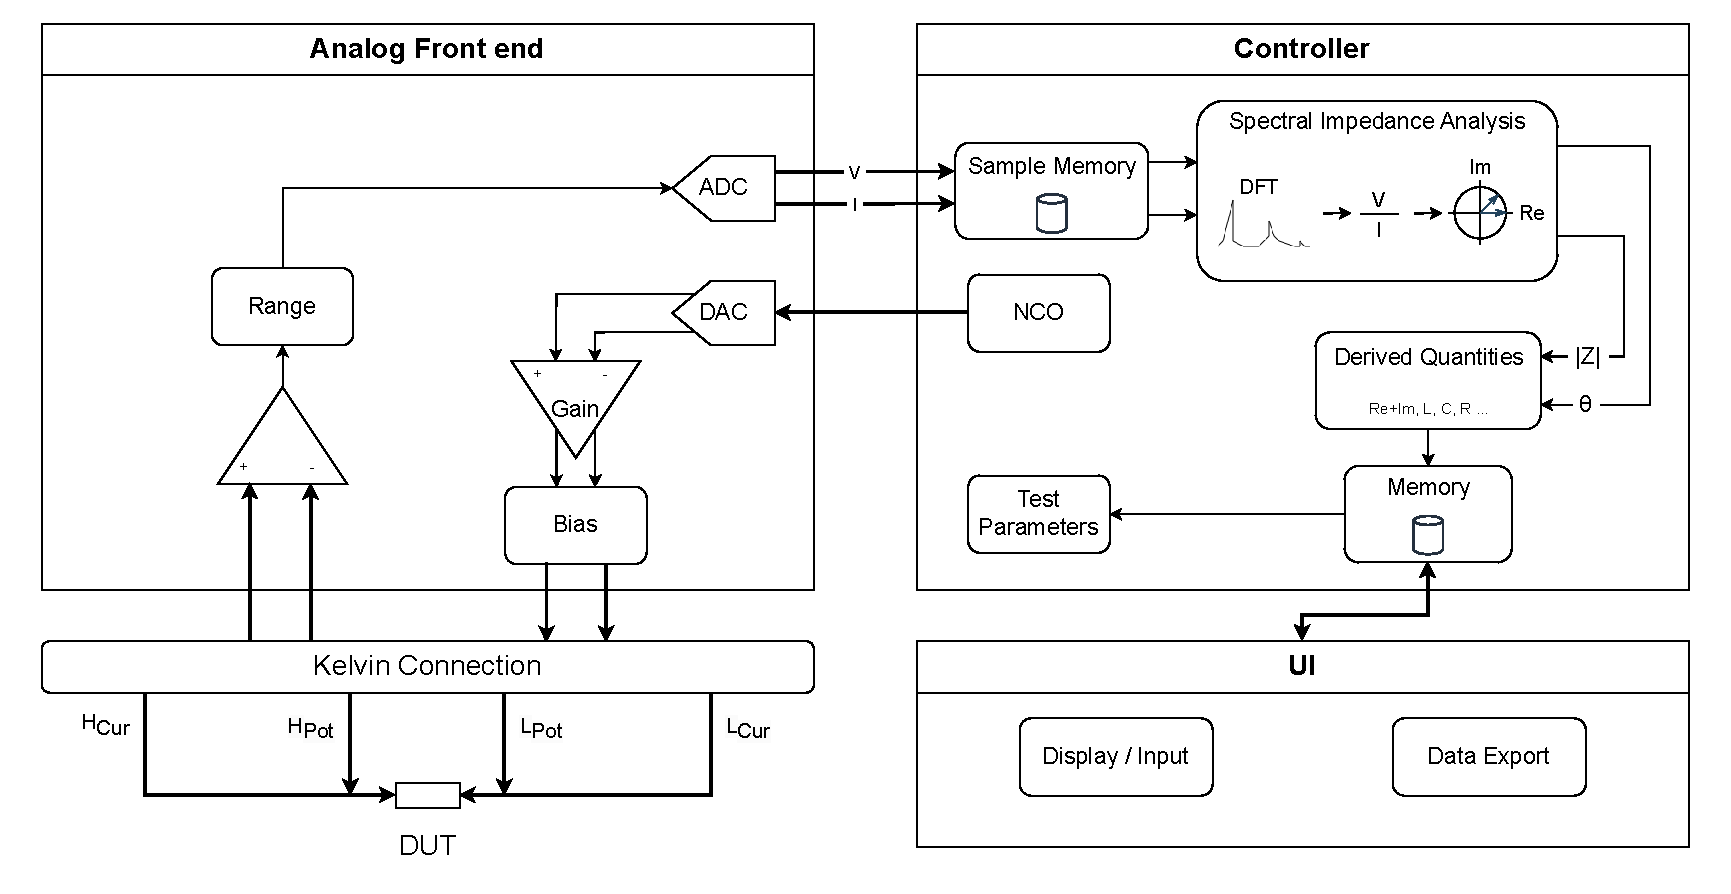
\includegraphics[clip, trim=18 0 18 0,width=1.0\textwidth]{Sections/6_SystemArchitecture/Figures/SystemArchitecture.pdf}
    \caption{The proposed system architecture for the impedance analyzer designed in this document. An analog front end will measure DUT voltage and current, 
    this will then undergo spectral analysis, such that phase and magnitude information can be obtained and used to calculate all derived quantities. A user can set the test parameters using a UI, these parameters in turn will determine DAC settings, range and sample rate.}
    \label{fig_6_SysArchitecture}
\end{figure}

The heart of the impedance analyzer lies in the Analog Front End whose purpose is to generate the test signals through DA-conversion while simultaneously acquiring the resulting DUT voltage and DUT current waveforms with AD-conversion. The DA- and AD-conversion is controlled by a sample control system. The sample control system will generate the required inputs for the DAC and it will take the samples from the two AD-converters and store them in sample memory. The sample control system will interface with a main processor. The main processors primary purpose is to retrieve the samples from the sample memory and perform all the necessary calculations on those samples in order to get the derivived quantities described in section \refq{subsec:DerivedQuantities}. When it has done the calculations it will transmit the results to a user interface; a display. The user interface will let the user set the test parameters, through a touch screen, and it will display the test results to the user.

The project team have discussed, extensively, the choice of digital platform and architecture for this system before arriving at the FPGA and Microprocessor combo shown on figure \refq{fig_6_SysArchitecture}. These considerations can be seen in appendix \refq{App:MicrocontrollerConsiderations}.

The system architecture on figure \refq{fig_6_SysArchitecture} has been split into separate modules in order to develop them in parallel. Each of the modules will be described in detail in the following subsections along with their specifications and required interfaces.
